\section{Ingwer-Curry}
% Linke Seite: Rezept
Zutaten (ca. 6 Portionen):
\begin{itemize}
    \item 2 rote Zwiebeln
    \item 1 Knoblauchzehe
    \item 3 cm Ingwer-Knolle
    \item 400g gelbe oder rote Linsen
    \item 3 Dosen geschälte Tomaten
    \item Curry-Pulver
    \item Salz und Pfeffer
    \item (Beilage) Jasmin-Reis
\end{itemize}

\noindent Zubereitung:

\noindent Linsen mit Wasser (1:2) in Gemüsebrühen in einem größeren Topf
aufkochen und ziehen lassen.

\noindent Gleichzeitig Ingwer, Zwiebeln und Knoblauch klein schneiden und mit 1
El Öl und 1-2 El Curry-Pulver in einem anderen Topf anbraten. Dann etwa 5
Minuten bei mittlerer Hitze zugedeckt anschwitzen lassen. Regelmäßig umrühren,
damit nichts anbrennt! Dann Tomaten hinzugeben, verrühren, und aufkochen
lassen. Tomaten-Mischung zu den Linsen geben und umrühren. Mit Salz und Pfeffer
abschmecken. Mit Reis servieren.

\noindent \textbf{Schmeckt auch gut mit Hummus und Reis in Tortillas!}

% Recht Seite: Bild
\newpage
\mbox{}
\vfill
\begin{center}
    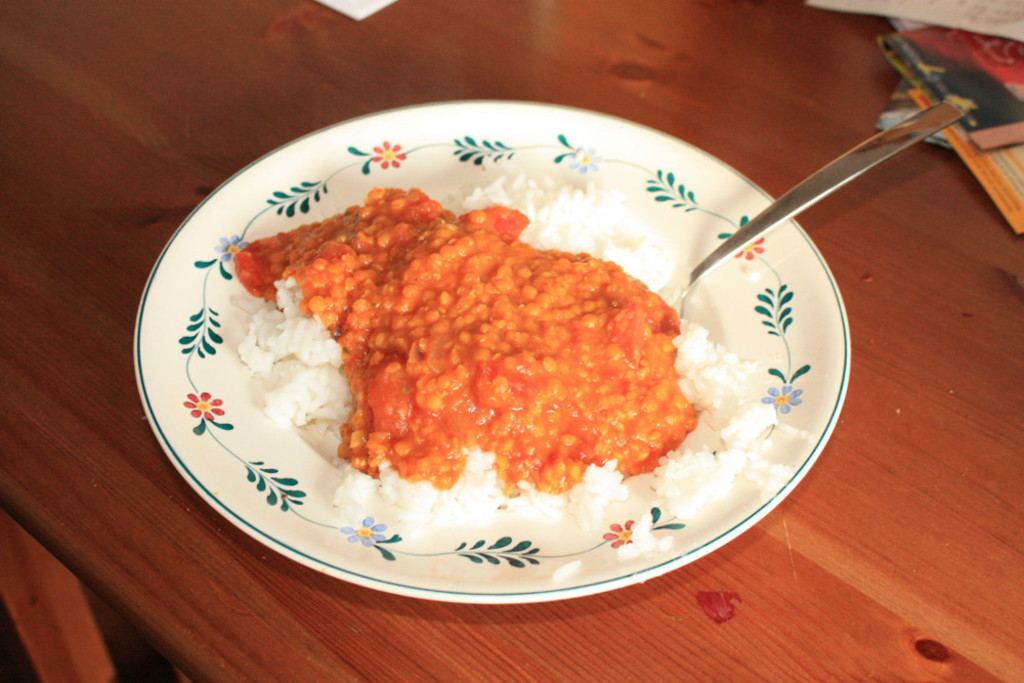
\includegraphics[width=\textwidth]{Ingwer-Curry/IMG_6088._small.jpg}
\end{center}
\vfill
\mbox{ }
\newpage
